\documentclass[tikz,border=2pt]{standalone}
\usepackage{amsmath}
\usepackage{pgfplots}
\pgfplotsset{compat=1.18}
\usetikzlibrary{arrows.meta}
\begin{document}
% Complete acceptance with threshold T = 2 for x_k = 1, s = (3,2,2,1,3,1,2,1):
% uncontrolled waits W = (0,2,3,4,4,6,6,7); controlled waits (0,2,3,2,2,4,3,2) with jobs 3, 6, 7 rejected.
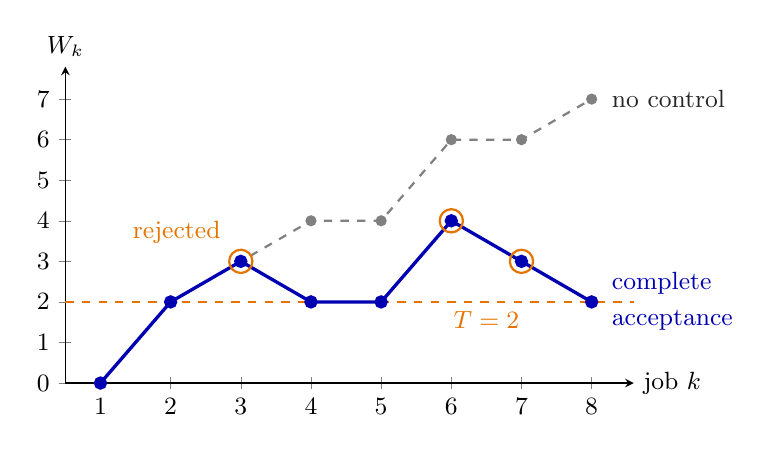
\begin{tikzpicture}[font=\small, >={Latex[length=2mm]}]
  \begin{axis}[
    axis lines=left, xmin=0.5, xmax=8.6, ymin=0, ymax=7.8,
    xtick={1,...,8}, ytick={0,1,...,7},
    xlabel={job $k$}, ylabel={$W_k$},
    xlabel style={at={(axis description cs:1,0)}, anchor=west},
    ylabel style={rotate=-90, at={(axis description cs:0,1)}, anchor=south},
    width=8.8cm, height=5.6cm, clip=false
    ]
    \draw[orange!90!black, thick, dashed] (axis cs:0.5,2) -- (axis cs:8.6,2);
    \node[orange!90!black, anchor=north] at (axis cs:6.5,2) {$T=2$};
    \addplot[gray, thick, dashed, mark=*, mark size=1.6pt, mark options={solid, fill=gray}]
      coordinates {(1,0) (2,2) (3,3) (4,4) (5,4) (6,6) (7,6) (8,7)};
    \addplot[blue!70!black, very thick, mark=*, mark size=1.8pt]
      coordinates {(1,0) (2,2) (3,3) (4,2) (5,2) (6,4) (7,3) (8,2)};
    \draw[orange!90!black, thick] (axis cs:3,3) circle (4.2pt);
    \draw[orange!90!black, thick] (axis cs:6,4) circle (4.2pt);
    \draw[orange!90!black, thick] (axis cs:7,3) circle (4.2pt);
    \node[orange!90!black, anchor=south east] at (axis cs:2.85,3.2) {rejected};
    \node[gray!30!black, anchor=west] at (axis cs:8.15,7) {no control};
    \node[blue!70!black, anchor=west] at (axis cs:8.15,2.45) {complete};
    \node[blue!70!black, anchor=west] at (axis cs:8.15,1.55) {acceptance};
  \end{axis}
\end{tikzpicture}
\end{document}
